\documentclass[tikz,border=6pt]{standalone}
% Native vector figure style. Okabe-Ito-derived colors; labels remain readable
% without color. Figure meaning must never depend on color alone.
\usepackage[T1]{fontenc}
\usepackage{helvet}
\renewcommand{\familydefault}{\sfdefault}
\hyphenpenalty=10000
\exhyphenpenalty=10000
\usepackage{tikz}
\usetikzlibrary{arrows.meta,positioning,fit,backgrounds,calc}
\definecolor{paBlue}{HTML}{0072B2}
\definecolor{paOrange}{HTML}{E69F00}
\definecolor{paGreen}{HTML}{009E73}
\definecolor{paPurple}{HTML}{CC79A7}
\definecolor{paInk}{HTML}{263441}
\tikzset{
  block/.style={draw=paInk,line width=.65pt,rounded corners=2pt,
    align=center,text=paInk,font=\sffamily\fontsize{9}{11}\selectfont,
    minimum height=1.15cm,text width=3.0cm,inner sep=5pt,fill=white},
  cpu/.style={block,fill=paBlue!10},
  memory/.style={block,fill=paOrange!13},
  compute/.style={block,fill=paGreen!10},
  control/.style={block,fill=paPurple!12},
  link/.style={-{Latex[length=2mm]},draw=paInk,line width=.8pt},
  duplex/.style={{Latex[length=2mm]}-{Latex[length=2mm]},draw=paInk,line width=.8pt},
  streaming/.style={duplex,draw=paBlue,line width=1.15pt},
  boundary/.style={draw=paInk!65,dashed,line width=.65pt,rounded corners=4pt},
  note/.style={font=\sffamily\fontsize{8}{10}\selectfont,align=center,text=paInk},
}

\begin{document}
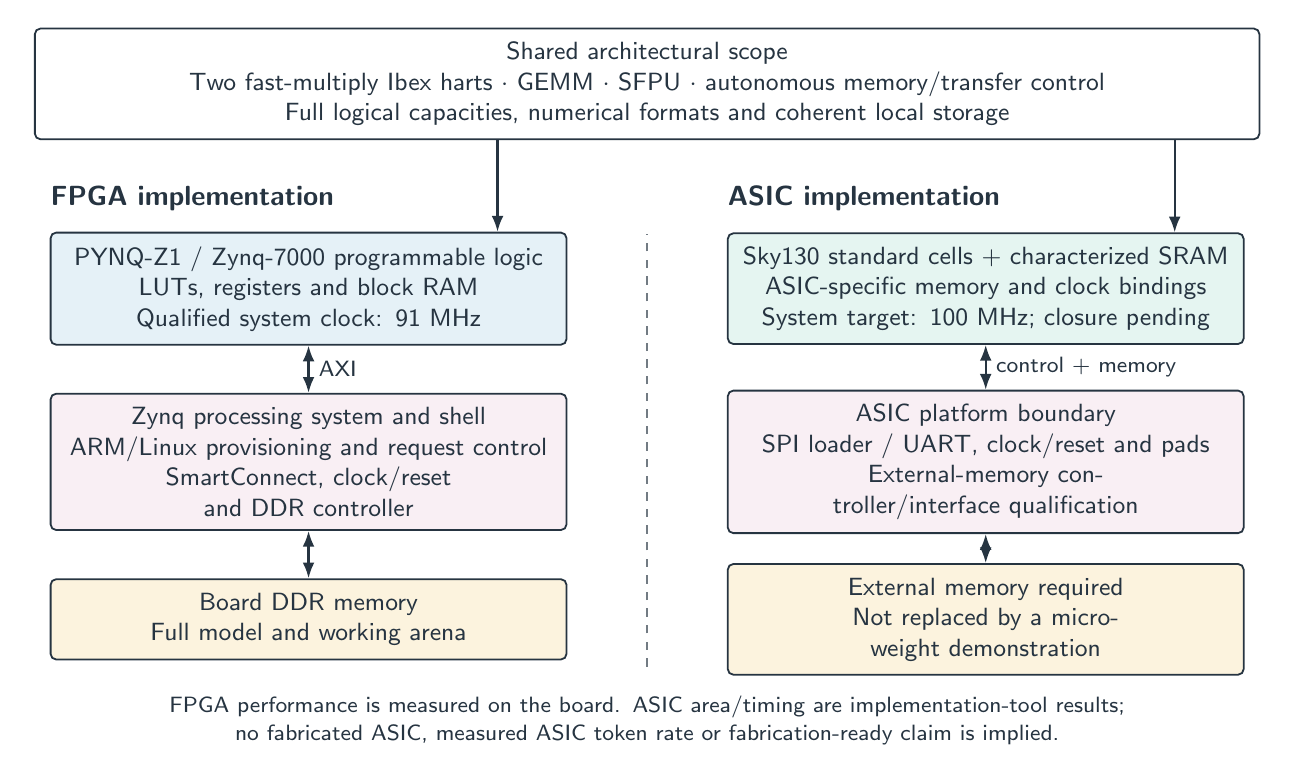
\begin{tikzpicture}[x=1cm,y=1cm]
  \node[block,text width=15.2cm,minimum height=1.3cm] (shared) at (7.9,7.5)
    {Shared architectural scope\\Two fast-multiply Ibex harts $\cdot$ GEMM $\cdot$ SFPU $\cdot$
     autonomous memory/transfer control\\Full logical capacities, numerical formats and coherent local storage};
  \node[note,anchor=west,font=\sffamily\bfseries\fontsize{10}{12}\selectfont] at (.2,6.05)
    {FPGA implementation};
  \node[note,anchor=west,font=\sffamily\bfseries\fontsize{10}{12}\selectfont] at (8.8,6.05)
    {ASIC implementation};
  \node[cpu,text width=6.2cm] (fpga) at (3.6,4.9)
    {PYNQ-Z1 / Zynq-7000 programmable logic\\LUTs, registers and block RAM\\Qualified system clock: 91 MHz};
  \node[compute,text width=6.2cm] (asic) at (12.2,4.9)
    {Sky130 standard cells + characterized SRAM\\ASIC-specific memory and clock bindings\\System target: 100 MHz; closure pending};
  \coordinate (fpgaentry) at ($(fpga.north)+(2.4,0)$);
  \coordinate (asicentry) at ($(asic.north)+(2.4,0)$);
  \draw[link] (shared.south -| fpgaentry) -- (fpgaentry);
  \draw[link] (shared.south -| asicentry) -- (asicentry);
  \node[control,text width=6.2cm] (ps) at (3.6,2.7)
    {Zynq processing system and shell\\ARM/Linux provisioning and request control\\SmartConnect, clock/reset and DDR controller};
  \node[control,text width=6.2cm] (chip) at (12.2,2.7)
    {ASIC platform boundary\\SPI loader / UART, clock/reset and pads\\External-memory controller/interface qualification};
  \draw[duplex] (fpga.south) -- node[note,right] {AXI} (ps.north);
  \draw[duplex] (asic.south) -- node[note,right] {control + memory} (chip.north);
  \node[memory,text width=6.2cm,minimum height=.85cm] (dram0) at (3.6,.7)
    {Board DDR memory\\Full model and working arena};
  \node[memory,text width=6.2cm,minimum height=.85cm] (dram1) at (12.2,.7)
    {External memory required\\Not replaced by a micro-weight demonstration};
  \draw[duplex] (ps.south) -- (dram0.north);
  \draw[duplex] (chip.south) -- (dram1.north);
  \draw[boundary] (7.9,.1) -- (7.9,5.6);
  \node[note,anchor=north,text width=15.5cm] at (7.9,-.15)
    {FPGA performance is measured on the board. ASIC area/timing are implementation-tool results;\\
     no fabricated ASIC, measured ASIC token rate or fabrication-ready claim is implied.};
\end{tikzpicture}
\end{document}
